\documentclass[titlepage,danish]{article}

\usepackage{fullpage}
\usepackage[utf8x]{inputenc}
\usepackage[danish]{babel}
\usepackage{color}
\usepackage{amssymb}
\usepackage{amsmath}
\usepackage{fancyhdr}
\usepackage{lastpage}
\usepackage{graphicx}
\usepackage{hyperref}
\usepackage{url}

\pagestyle{fancy}
\fancyhf{}
\setlength{\headheight}{15pt}
\setlength{\headsep}{25pt}
\lhead{Kursus 02121}
\chead{Space Invaders}
\rhead{s113491, s123692, s123563}
\lfoot{\thepage{} af \pageref{LastPage}}
\rfoot{20/01-2013}

% use when representing code and file names
\newcommand{\code}[1]{\texttt{#1}}

\begin{document}

\title{Space Invaders (kursus 02121)}
\date{20/01-2013}
\author{
  Gadd, Patrick\\
  \texttt{s113491}
  \and
  Veie Færgevaa, Markus\\
  \texttt{s123692}
  \and
  Altschuler, Simon\\
  \texttt{s123563}
}
\maketitle

\section{Afgrænsning}
\emph{Her beskrives hvordan afgrænsnings processen foregik og hvad resultatet var.}\\*
Vi vidste fra starten at det er umuligt at vide præcist hvor langt man kan nå i et givent
tidsrum. Derfor var mentaliteten hele tiden at udvikle programmet på så generisk vis som muligt,
således at det ville være nemt at udbygge med nye features, og det uden at koden bliver såkaldt
``slamkode'' (dvs. uorganiseret, dårlig performance, uoverskueligt, etc). Dette er også en af
softwareudviklingens tommelfingerregler: ``It's gonna change''.

Derfor har vi forsøgt at holde koden DRY \footnote{Don't Repeat Yourself
  \url{http://en.wikipedia.org/wiki/Don't_repeat_yourself}}, velstruktureret, i henhold til bevist
velfungerende design principper, osv.

Et par features som vi dog vidste at vi ville/skulle nå at implementere:
\begin{description}
  \item[Klassisk Space Invaders gameplay] \hfill \\
    Hermed menes ``forsinkede'' skud, bevægende invaders som skyder tilbage, bunkers og den slags.

  \item[Menu system] \hfill \\
    Et system til at vise og styre forskellige skærme (såsom menu, selve spillet, game over,
    highscore), samt et system til at oprette disse på en simpel måde.

  \item[Highscores] \hfill \\
    Et highscore system (som blev implementeret gennem en web service vi også udviklede, således at
    highscoren er global).

\end{description}

Derfor brugte vi de første dage på at udvikle arkitekturen og gennemtænke hvordan tingene skulle
sættes passende sammen. Derefter begyndte vi at udvikle specifikke dele af programmet, og her blev
det også meget nemmere at dele opgaver ud, da delene som regel var fuldstændig uafhængige og dermed
nemt kunne udvikles seperat.

Dette leder til programmets egentlig implementation.

\section{Implementation}
\emph{Her beskrives spillets strukturelle opbygning, samt vigtige konkrete implementeringsstrategier}
\subsection{Overordnet struktur}
Programmet er opbygget med den klassiske MVC arkitektur som hovedprincip. MVC er blevet brugt og
beskrevet så meget at det næsten kan siges at være blevet en kliché. Det er umuligt at definere helt
præcist hvordan en egentlig korrekt implementering ser ud (fordi den ikke findes), men de
overordnede princippet gælder mere eller mindre for alle varianter. Disse principper inkluderer
f.eks. at controller ``snakker med'' model og view og dermed agerer mellemmand mellem de to, og at
view og model ikke kommunikerer direkte. Sidstenævnte bryder vi en smule, idet vi bruger Observer
pattern.

I vores tilfælde har vi en \code{MainController}, \code{MainView} og \code{MainModel}. Udover det
bruger vi Command pattern til at facilitere eksekvering af ``cachet'' logik, og Observer pattern til
at opdatere views når modellen ændres. Vi gennemgår kort nogle vigtige klasser og principper:

\begin{description}
\item[\code{MainController}] \hfill \\
  Den overordnede controller, som holder instanser af sub-controllers og ikke laver noget egentligt
  arbejde selv. Pointen er, at har man en reference til \code{MainController}, kan man tilgå alle
  andre controllers som getters på denne. Dette gør det nemt og bekvemt at kalde forskellige sub
  controller metoder fra forskellige steder uden at skulle sende hver enkel controller rundt for
  sig.

\item[\code{MainView}]  \hfill \\
  Det øverste view, hvori alle andre views bliver renderet. \code{MainView} indeholder på ethvert
  givent tidspunkt én instans af \code{AbstractViewState}, som bliver renderet i vinduet. Denne
  sættes gennem en Command som kalder en metode på \code{StateController}.

\item[\code{MainModel}]  \hfill \\
  Den overordnede model. Heri ligger al data som beskriver programmets nuv�rende tilstand. Dette
  inkluderer alt fra hvor stort hovedvinduet er, til hvornår man sidst har affyret et skud. Al data
  som er en del af en specifik spille-session (dvs, hvor mange invaders er der, hvor er de, hvorn�r
  blev spillet sidst opdateret og renderet), bliver gemt i et \code{GameState} object. Dette gemmes
  i \code{MainModel} som det aktive spille-sessions state. Dette object er d�t som bliver givet til
  en \code{GameController}, der s� opdaterer det og sender det til rendering.

\item[\code{Command}s] \hfill \\
  \code{Command}s bliver brugt til at enkapsulere logik der \emph{kan v�re} afhængig af state. Denne
  logik kan så efterfølgende eksekveres af hvem som helst, når som helst, uden at denne har nogen
  viden om hvad en given \code{Command} \emph{egentlig} gør. Fælles for dem alle er at implementerer
  \code{ICommand} interfacet, hvilket består af en enkelt metode: \code{execute}.  Det er specielt
  bekvemt til f.eks. at eksekvere logik ved tryk på knapper (hvor knappen ikke skal vide hvad den
  laver), men også til generelt at lagre og udføre logik fra andre steder.  Vi har det klassiske
  command pattern en smule ved at implementere en \code{chain} metode, som effektivt sætter
  \code{Command}s sammen i rækkefølge og returnerer en ny command.

\item[Observers] \hfill \\
  \code{MainModel} implementerer Java's \code{Observable}. Det er en måde for et object at eksponere
  et interface som gør et andet object, en \code{Observer}, opmærksom på hvornår den er
  opdateret. Vha. observer pattern gøres dette fuldstændig decoupled, og \code{MainModel} har altså
  ingen ide om hvem der lytter efter dens ændringer. Ændringerne annonceres gennem
  \code{Oberservable}s \code{notifyObservers} metode.
\end{description}

Vi har valgt ikke at udvikle tests til projektet. Vi kunne have lavet en masse Unit Tests som kunne
have fanget fejl for os, eller endda udviklet i TDD stil. Vi vurderede dog at til et projekt af
denne størrelse og art at det ikke ville være det værd. I stedet har vi været grundige for at
udvikle i en stil der forebygger fejl.

\subsection{GameController}
Står primært for at opdatere \code{GameState} samt at få \code{GameStateRenderer} (kaldet renderer
under \code{GameController}) til at rendere \code{GameState}. Derudover anvendes en
\code{javax.swing.Timer} som game loop opdaterings trigger. Timeren eksekverer en
\code{UpdateGameStateCommand} ved hver trigger.

Metoden \code{updateGameState()} gør følgende (i kronologisk rækkefølge):
\begin{enumerate}

\item \code{currentTime} bruges til at udregne \code{timeDelta}, gemmes i det aktuelle
  \code{GameSate} så man kan se hvornår det sidst blev opdateret, samt til at afgøre om
  \code{Player} og \code{Invaders} må skyde i denne update.

\code{timeDelta} bruges til at bevæge samtlige \code{GameElement}’er afhængigt af den tid der er gået, sådan at de for spilleren bevæger sig med konstant hastighed uafhængigt af om tiden mellem updates varierer.

\item Kontrollerer om \code{GameStateState} er \code{Running}/\code{Waiting}/\code{Paused}. Hvis denne enum er \code{Waiting}/\code{Paused} returnerer metoden og kører dermed ikke videre. Hvis den er running fortsætter den og tjekker om spilleren eventuelt trykker ESC for at pause (og returnere).

\item Herefter bliver alle \code{GameElement}’erne opdateret. Dette indebærer at der bliver tjekket med utils.Input om en listener er aktiveret af spilleren, rykke relevante elementer, kontrollere for kollisioner og endeligt fjerne de elementer der er blevet mærket "døde".

\item Tjekker om man har vundet/tabt og returnerer hvis dette er tilfældet. Kalder \code{GameStateRenderer.render()} og renderer hermed det aktuelle \code{GameState}.

\item Kalder \code{GameStateRenderer} og får denne til at rendere det aktuelle \code{GameState}. \emph{Simon: Vi burde teoretisk set nok have haft en overordnet klasse (Nogle bud???) som kaldte \code{updateGameState()} og \code{GameStateRenderer.render()} uafhængigt af hinanden, sådan at \code{GameState} kunne opdateres uden at nødvendigvis blive renderet}

\item Slutteligt opdateres tiden gemt i \code{GameState}.
\end{enumerate}


\subsection{utils.Mathx}
Indeholder belejlige matematiske metoder, hvoraf den eneste rigtigt interessante er
\code{circleRectangleIntersects()}, som er noget mere advanceret end detektion mellem
rektangel-rektangel eller cirkel-cirkel. Den ser således ud:

\begin{verbatim}
boolean circleRectangleIntersects(GameElement rect, Coordinate circ, double radius){

  double rectCenterX = rect.getPosition().x + ((double) rect.getWidth()/2);
  double rectCenterY = rect.getPosition().y + ((double) rect.getHeight()/2);

  double circleDistanceX = Math.abs(rectCenterX-circ.x);
  double circleDistanceY = Math.abs(rectCenterY-circ.y);

  if (circleDistanceX > (rect.getWidth()/2 + radius)) { return false; }
  if (circleDistanceY > (rect.getHeight()/2 + radius)) { return false; }
}
\end{verbatim}

De to ovenstående \code{if} conditionals har udelukket alle tilfælde hvor cirklen ligger udenfor en
forstørret udgave af rektanglen (rektanglen + radius). Dette svarer til det lyserøde område på
figur \ref{fig:col_rect}.

\begin{figure}[h!]
  \centering
  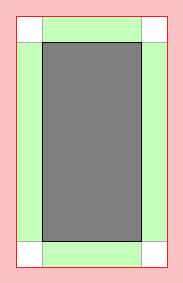
\includegraphics[scale=0.60]{rekt_cirk_02.png}
  \caption{Farverne repræsenterer de forskellige tjek som bliver udført i funktionen \code{circleRectangleIntersects}}
  \label{fig:col_rect}
\end{figure}

Derfor vil cirklen ligge indenfor rektanglen+(cirklens radius) for de to nedenstående \code{if}
conditionals. Disse to tjekker om cirklens centrum ligger i de på illustrationen lysegrønne områder,
eller ligefrem indenfor rektanglen (mørkegrå).
\begin{verbatim}
    if (circleDistanceX <= (rect.getWidth()/2)) { return true; } 
    if (circleDistanceY <= (rect.getHeight()/2)) { return true; }
\end{verbatim}	    
Tilbage er der kun at kontrollere hjørnerne af den forstørrede rektangel (kvadrater med cirklens
radius som sidelængde). Dette svarer til de hvide områder på figur \ref{fig:col_rect}.
\code{cornerDistanceSquared} er cirklens centrums afstand til den oprindelige rektangels hjørner
kvadreret.
\begin{verbatim}
    double cornerDistanceSquared = Math.pow((circleDistanceX - rect.getWidth()/2),2) + 
        Math.pow((circleDistanceY - rect.getHeight()/2), 2);
    return (cornerDistanceSquared <= Math.pow(radius,2));
}
\end{verbatim}
Er cirklens centrum længere væk end dens radius er der ikke kollision.

\section{Evaluering}
\emph{Vi evaluerer process og resultat af arbejdet.}
\subsection{Process}
Vores udviklingsprocess viste sig at fungere godt. Versionsstyring er guld værd, og den eneste
ulempe vi fandt ved git er at det kan betale sig at holde styr på hvem der arbejder hvor, for at
undgå for meget merging arbejde.

Lige i starten var alle med til sammen at udtænke den overordnede opbygning, men som fundamentet
efterhånden blev lagt, kunne vi dele arbejdet op i isolerede opgaver som man individuelt fik ansvar
for at implementere. Denne fremgangsmåde virkede godt, og var meget effektiv, både fordi det var
nemt at projektstyre, og fordi vi hver især fik lyst til at levere et godt stykke arbejde.

Samarbejdet har været godt, alle har arbejdet lige har sat deres præg på resultatet. Alle har været
gode til at sætte sig ind i, og respektere andres arbejde.

\subsection{Samlet result}
Vi er meget tilfredse med hvordan resultatet blev. Det gik hurtigere og hurtigere at få
implementeret nyt features, i takt med at vi vænnede os til strukturen, og den viste sig at holde
til de udvidelser vi havde i sinde.

Det betalte sig på alle måder at lave spillet generisk nok til at det ikke var designet med et helt
konkret feature sæt i sinde. Det har været nemt og bekvemt at udvikle forskellige dele af spillet
samtidig, også selvom vi har pushet og pullet ofte. 

\subsection{Videre udvikling}
En ting vi burde lærer at blive bedre til er at rebase og håndterer commits, for vi endte ofte med
at pushe 5 commits ad gangen, hvoraf de 4 var merge commits af branches og conflict
resolutions. Vores hoved repository endte op med alt for mange commits, så det ville være svært, i
nogle tilfælde, at snævre en feature ned til et bestemt commit i timelinen.

Hvis vi skulle arbejde videre med projektet ville næste skridt være at strømline al kode, og
derefter lave tests, for at sikre stabilitet.

\section{Værktøjer}
\emph{Kort gennemgang af de værktøjer vi har brugt}
\subsection{Versionsstyring}
Til projektet har vi brugt git\footnote{git: \url{http://git-scm.com}}. Det har visse fordele over
f.eks. SVN og Mercurial (og specielt TFS). Kort opsummering af grunde til at bruge git:

\begin{description}
  \item[Distribueret] \hfill \\
    git er en af de eneste fuldstændig distribuerede VCS'er. Man arbejder altid i sit eget lokale
    repository, og kan gøre hvad man vil, uafhængigt af alle andre. Man har så et hostet
    \emph{main} repository, som regel kaldet origin, som vi hoster på GitHub \footnote{GitHub:
      \url{http://github.com}}. 

    En fremragende følge af dette er at alle kan arbejde uden netforbindelse, og da et commit bliver
    committet lokalt går det \emph{meget} hurtigere, da der ikke skal forbindes til server.

  \item[Branching] \hfill \\
    Branching er meget mere ligetil i git i forhold til SVN og Mercurial, og skift af branch samt
    merge af disse er intuitivt og nemt.

  \item[Performance og størrelse] \hfill \\
    git er utroligt hurtigt, og utrolig god til at kompresse data (til sammenligning fylder Mozillas
    samlede repo med commit historie 12gb i SVN og noget ala 400mb i git!).
\end{description}

\subsection{IDE}
Som IDE har vi brugt både Eclipse\footnote{Eclipse:\url{http://www.eclipse.org}} og
NetBeans\footnote{NetBeans: \url{http://www.netbeans.org}}. De to minder meget om hinanden, er begge
open source og valget er en smagssag. Begge har de også integration af versionsstyring, hvor vi dog
har holdt os til command-line git, da den slags GUI værktøjer som regel er lidt ustabile.

\subsection{Diverse}
Vi har brugt Paint.NET\footnote{Paint.NET: \url{http://www.getpaint.net}} til at redigere grafik, og
Audacity til lydredigering\footnote{Audacity: \url{http://audacity.sourceforge.net}}.

\end{document}